Introduzione alla sezione


\subsection{Sensori}
\label{ssez:sensori}

Descrizione di quelli utilizzati e confronto con gli altri.

  \subsection{Gli accelerometri} \label{ssez:accelerometri}
    Specifiche richieste (in ordine di priorità):
	\begin{itemize}
      \item [] {Uscita digitale}
	  \item [] {Accelerazione massima $\ge \pm8g$}
      \item [] {Frequenza di campionamento $\geq 100Hz$}
      \item [] {Digitalizzazione a profondità $\ge 8bit$}
      \item [] {Almeno due indirizzi disponibili}
      \item [] {Prezzo $\le$ 20\euro}
	\end{itemize}

    La \textsc{Tabella~\ref{tab:accelerometri}} mostra sinteticamente un confronto
    tra i sensori disponibili sul mercato.

	\begin{table}
		% Center the table
		\begin{center}
		% Title of the table
		\caption{Confronto tra gli accelerometri da acquistare}
		\label{tab:accelerometri}
		% Table itself: here we have two columns which are centered and have lines to the left, right and in the middle: |c|c|
		\begin{tabular}{r c c c c}
			% To create a horizontal line, type \hline
%			\hline
			% To end a column type &
			% For a linebreak type \\
Disp.  & Range ($\pm$g) & Codifica (bit) & Prezzo (\euro) & Interfaccia \\
			\hline
InvSen & 2-16           & 16         & 18,00          & \iic \\
mCube  & 2-16           & 8-14       & 11,32          &\iic, {\relsize{-1} SPI} \\
\textbf{AdaF} & \textbf{2-8} & \textbf{14} & \textbf{9,31} & \textbf{\iic} \\
SF MMA & 2-8            & 8, 12      & 10,03          & \iic \\
\textbf{ADXL345} & \textbf{2-16} & \textbf{10-13} & - & \textbf{\iic,{\relsize{-1} SPI}} \\
			\hline
		\end{tabular}
		\end{center}
	\end{table}
    
    \subsubsection {L'uscita digitale} \label{sssez:digitale}	
    Con l'uscita digitale, per ogni numero di accelerometri
    è sufficiente un unico \textit{bus} da tre cavi
	\footnote{\,Dipende da quanti indirizzi sono disponibili
	(vedi: \textsc{\ref{sssez:indirizzi}})}:
	dati, clock e massa;
    con l'uscita analogica è
\[
	cavi = accelerometri \times assi
\]
    quindi per quattro accelerometri triassiali occorrono
    \(4 \times 3  = 12\) cavi.
    A tanti cavi corrisponderebbero tanti ingressi analogici di microcontrollore.
    

    \subsubsection {Ampiezza e frequenza di campionamento} \label{sssez:accmax}
    Per determinare quale fosse l'ampiezza minima necessaria,
    sono stati usati due accelerometri già disponibili:
    il primo è all'interno di un telefono cellulare {\relsize{-1} GT-S7501};
    il secondo fa parte di un sistema di acquisizione professionale.
    Un sintetico confronto in {\relsize{-.5} \textsc{Tabella~\ref{tab:accelerometricasa}}}.
    Entrambi sono stati sottoposti a movimenti semplici e
    al lancio di un dardo.
	\begin{table}
		% Center the table
	  \begin{center}
		% Title of the table
		\caption{Confronto tra gli accelerometri già disponibili}
		\label{tab:accelerometricasa}
		% Table itself: here we have two columns which are centered and have lines to the left, right and in the middle: |c|c|
		\begin{tabular}{r c c}
			% To create a horizontal line, type \hline
%			\hline
			% To end a column type &
			% For a linebreak type \\
Disp.   & Range ($\pm$g) & Freq. Camp. (Hz)\\
			\hline
GT-S750 & 2              & 50 \\
Pro     & $>$30          & 10k \\
			\hline
		\end{tabular}
	  \end{center}
	\end{table}
        
    L'accelerometro di fascia bassa risponde adeguatamente a sollecitazioni deboli,
    mentre risulta totalmente inadeguato all'applicazione finale,
    sia per ampiezza che per frequenza di campionamento.
    Prima di ricorrere all'accelerometro professionale,
    si è cercato di ricostruire il segnale corrotto dalla saturazione.
    In \textsc{Figura~\ref{fig:ricostruzione}}
    il segnale da ricostruire è rappresentato in blu e
    in rosso il segnale corretto, mentre
    con il bollino nero si evidenzia l'ampiezza massima stimata.
    A posteriori, si vedrà che il segnale vero è più ampio.
    Si nota presto che la frequenza di campionamento
    dev'essere almeno raddoppiata.

%	\textbf{Cercare di standardizzare il grafico in b/n,
%		con i bollini e la legenda, e soprattutto in {\relsize{-.5} EPS}}.

% This is how you include a eps figure in your document. LaTeX only accepts EPS or TIFF files.
	\begin{figure}
		% Center the figure.
		\begin{center}
		% Include the eps file, scale it such that it's width equals the column width. You can also put width=8cm for example...
		\includegraphics[width=\columnwidth]{taybella_copia}
		% Create a subtitle for the figure.
		\caption{Esempio di ricostruzione di un segnale saturato}
		% Define the label of the figure. It's good to use 'fig:title', so you know that the label belongs to a figure.
		\label{fig:ricostruzione}
		\end{center}
	\end{figure}

	Con l'accelerometro di fascia alta si è invece potuto acquisire
    il vero movimento; da questo si sono ricavate le specifiche
    sugli accelerometri.
    
    
	\subsubsection {Indirizzi} \label{sssez:indirizzi}
    Come sarà spiegato in maggior dettaglio nella \textsc{Sezione~\ref{sez:protocollo_i2c}}
    il protocollo {\iic} richiede che in un determinato istante
    un dispositivo faccia da {\master} e gli altri da {\slave}.
    
    Concettualmente il calcolatore è {\master}
    \footnote{\,Il calcolatore non comunica direttamente sul \textit{bus} {\iic},
    quindi il vero {\master} è il processore del convertitore}
    e gli accelerometri sono {\slave}.
    All'inizio di ogni nuova comunicazione il \master{}
    scrive sul \textit{bus} l'indirizzo dello \textit{slave} interrogato.
    Il messaggio è lungo un byte ed è formato da 7 bit di indirizzo
    seguiti dal bit di comando: \texttt{1}\,=\,lettura e \texttt{0}=scrittura.
    
Il protocollo \iic{} mette quindi a disposizione
    \(2^7=128\) indirizzi \footnote{\,Sedici indirizzi sono riservati}
    ma i costruttori delle schede di sviluppo su cui sono montati gli accelerometri
    fissano tutti o quasi i piedini, lasciando disponibili uno o due indirizzi.
    Si rende quindi necessario l'utilizzo di linee separate o di un \textit{multiplexer}: avendo disponibile in casa un adattatore con due canali,
    si è scelto di percorrere la prima via.








\subsection{Trasmissione}
\label{ssez:trasmissione}



\subsection{Il convertitore I2C-USB}
%  	Descrizione di quello utilizzato e confronto con gli altri.
    Specifiche richieste:
	\begin{itemize}
	  \item Minimo due canali
	\end{itemize}

    \subsubsection{Due canali} \label{sssez:2canali}
    La specifica deriva dalle osservazioni del paragrafo precedente:
    si è scelto di usare quattro sensori con due soli indirizzi disponibili
    quindi è necessario utilizzare due linee o un \textit{multiplexer}.
    Il modulo di espansione \emph{\relsize{-.5}{FTDI-RPi}} mette a disposizione
    tre porte \usb{} e due canali seriali multiuso
    (a scelta tra \iic{}, {\relsize{-.5} UART} e seriale).
    I produttori forniscono anche le librerie {\relsize{-.5} C++} per l'interfacciamento.
    
	\begin{table}
		% Center the table
		\begin{center}
		% Title of the table
		\caption{Confronto tra i convertitori \iic-\usb}
		\label{tab:convertitori}
		% Table itself: here we have two columns which are centered and have lines to the left, right and in the middle: |c|c|
		\begin{tabular}{r c c}
			% To create a horizontal line, type \hline
%			\hline
			% To end a column type &
			% For a linebreak type \\
Disp.        & Canali (n)  & Prezzo (\euro)\\
			\hline
200XD        &  4          & 8,72\\
USB-ISS      &  1          & 24,89\\
\textbf{Rpi} &  \textbf{2} & \textbf{34,00}\\
			\hline
		\end{tabular}
		\end{center}
	\end{table}

% \input{rpihub.tex}

\section{Il protocollo I2C} \label{sez:protocollo_i2c}
{Nota: Tutta questa sezione fa riferimento alla guida~\cite{cit:primer}.}

\relsize{0}
%	Descrizione del protocollo con le solite figure.
    Fu progettato dalla Philips Semiconduttori (ora NXP) nel 1982
    per la comunicazione tra componenti sulla stessa scheda circuitale.
    La velocità standard è di 100kbit/s,
    accelerata a 400kbit/s (modalità veloce)
    oppure a 3,4Mb/s (alta velocità).
    A livello fisico le linee \sda{} e \scl{} sono a \emph{collettore aperto}
    (\textit{open-drain}),
    cioè possono essere forzate basse oppure \emph{lasciate} alte~\cite{cit:primer}.
	
\begin{figure}[t]
	\centering
	\includegraphics[scale=.3]{I2C_data_transfer}
    \caption{Diagramma temporale di una comunicazione \iic{}. S - Start; P - Stop; B - trasferimento di un bit; commutazione sul fronte di discesa del clock (blu). Opera di pubblico dominio di Marcin Floryan.}
    \label{fig:i2c_trans}
\end{figure}


    Pregi:
\begin{itemize}
	\item {sono necessarie soltanto due linee}
	\item {relazione {\master}-{\slave}, ciascuno con un indirizzo univoco}
	\item {il master genera il clock}
	\item {
    	possibilità di \textit{multimaster} tramite arbitraggio
   		\footnote {
        	non essendo utilizzato nel progetto,
        	questo aspetto non sarà trattato
        }
	}
\end{itemize}

\subsection{Considerazioni hardware}

\subsubsection{Configurazione tipica}
La \textsc{Figura \ref{fig:i2c_tipica}}
mostra la tipica configurazione di una linea {\iic}
con le resistenze $R_S$ in serie,
le resistenze $R_P$ di \pullup,
le capacità parassite $C_P$
e quella di \textit{crosstalk} $C_C$, di interferenza tra le linee.

Ciascun dispositivo può \footnote{\,dovrebbe poter}
intervenire soltanto abbassando la linea.

Le resistenze di {\pullup} possono essere inserite alla fine della linea
e per questo sono chiamate anche \textit{{\iic} termination};
hanno comunemente un valore di $1k\Omega$.

Le resistenze in serie possono essere molto basse o quasi nulle
a meno che non si abbia l'esigenza di proteggere il circuito da correnti esterne.
Per ogni dispositivo si considerano uguali le resistenze su {\sda} e {\scl}
\begin{equation}
	R_{S\,1,\,j}\,=\,R_{S\,2,\,j}\qquad \forall i.
\label{eqn:rs}
\end{equation}
Quando una linea è abbassata al livello logico \textsc{0},
la tensione è data dal partitore tra $R_P$ e $R_S$.
Per la linea $i$ comandata dal dispositivo $j$ è
\begin{align}
	V_{i}\,&=\,\frac{R_{S\,i,\,j}}{R_{S\,i,\,j}+R_{P\,i}}\;V_{CC} \\
    & =\,\frac{50}{50+1k}\;3.3V \,=\,157mV
\label{eqn:partitore}
\end{align}
La conseguenza positiva è che assegnando a ogni dispositivo un valore di $R_S$ differente,
è possibile per il progettista capire quale dispositivo sta agendo sulla linea.
Per contro, può accadere che questa tensione non sia abbastanza bassa da essere letta come \textsc{0} logico,
con le implicazioni descritte più avanti nel testo.

\begin{figure}
  \centering
  \resizebox{.9\linewidth}{!}{	\begin{tikzpicture}
\relsize{-1}
\node (nSDA1) at (-3,1) {};
\node (nSCL1) at (-3,-1) {};
\node (nSDA2) at (3,1) {};
\node (nSCL2) at (3,-1) {};
\node (nCondens1) at (0,1) {};
\node (nCondens2) at (0,-1) {};
\node (nPullUp1) at (-1,1) {};
\node (nPullUp2) at (1,-1) {};
\node (nFinto1) at (1,1) {};
\node (nFinto2) at (-1,-1) {};
\node (nAlimPullUp1) at (-1, 3) {};
\node (nAlimPullUp2) at (1, 3) {};
\node (nAlim1) at (-3, 3) {};
\node (nAlim2) at (3, 3) {};
\node (nMassaCap1) at (-1, -3) {};
\node (nMassaCap2) at (1, -3) {};
\node (nMassa1) at (-3, -3) {};
\node (nMassa2) at (3, -3) {};
\node (nSDAin1) at (-6, 1) {};
\node (nSDAout1) at (-6, 0) {};
\node (nSCLin1) at (-6, -1) {};
\node (nSCLout1) at (-6, -2) {};
\node (nSDAin2) at (6, 1) {};
\node (nSDAout2) at (6, 0) {};
\node (nSCLin2) at (6, -1) {};
\node (nSCLout2) at (6, -2) {};

%	
%	Resistenze in serie
\draw (nSDA1) to [resistor, l^=$R_{S11}$, o-, n=r11] (nPullUp1)
      (nSCL1) to [resistor, l^=$R_{S21}$, o-, n=r21] (nFinto2)
      (nFinto1) to [resistor, l^=$R_{S12}$, -o, n=r12] (nSDA2)
      (nPullUp2) to [resistor, l^=$R_{S22}$, -o, n=r22] (nSCL2);
%	
%	Resistori in parallelo
\draw (nAlimPullUp1) to [resistor, l^=$R_{P1}$, n=rp1] (nPullUp1)
      (nAlimPullUp2) to [resistor, l^=$R_{P2}$, n=rp1] (nFinto1);
%	
%	Condensatori
\draw (nCondens1) to [capacitor, *-*, n=cc] (nCondens2) 
      (nFinto1) to [short] (nPullUp2) to [capacitor, l^=$C_{P2}$, n=cp2] (nMassaCap2)
      (nPullUp1) to [short] (nFinto2) to [capacitor, l^=$C_{P1}$, n=cp2] (nMassaCap1);
\node at (.5,-.5) {$C_C$};
%	
%	Transistori
\draw (-3.5,-1) to [Tnmos=11, n=mos11] ++(0, 2)
	  (-4,-3) to [Tnmos=21, n=mos21] ++(0, 2);
\draw (3.5, 1) to [Tnmos=12, n=mos12] ++(0, -2)
	  (4,-1) to [Tnmos=22, n=mos22] ++(0, -2);
%	
%	Cortocircuiti
\draw (nPullUp1) to [short, *-] (nFinto1)
	  (nFinto2) to [short, -*] (nPullUp2);
\draw (-6,-3) to [short, -*] (-4,-3)
	  to [short] (nMassa1)
      to [short, o-*] (nMassaCap1)
	  to [short] (nMassaCap2)
      to [short, *-o] (nMassa2)
      to [short] (4,-3)
      to [short, *-] (6,-3);
\draw (-6, 3) to [short] (nAlim1)
	  to [short, o-*] (nAlimPullUp1) 
	  to [short] (nAlimPullUp2)
      to [short, *-o] (nAlim2) to [short] (6,3);
\draw (-3.5, -1) to [short, -*] ++(0,-2);
\draw (3.5, -1) to [short, -*] ++(0,-2);
\node (alim) [rground, yscale=-1] at (0, 3) {};
  \node [right] at (0,3.5) {$V_{CC}$};
\node (massa) [cground] at (0, -3) {};
%	
%	Segnali
\draw (nSDA1) to [short, -*] ++(-.5,0) to [short] (-5,1) to [short, i_=$SDA\,in$] (nSDAin1);
\draw (nSDAout1) to [short, i^=$SDA\,out$] (-5,0) to [short] (mos11.G);
\draw (nSCL1) to [short, -*] ++(-1,0) to [short] (-5,-1) to [short, i_=$SCL\,in$] (nSCLin1);
\draw (nSCLout1) to [short, i^=$SCL\,out$] (-5,-2) to [short] (mos21.G);
%	
\draw (nSDA2) to [short, -*] ++(.5,0) to [short] (5,1) to [short, i=$SDA\,in$] (nSDAin2);
\draw (nSDAout2) to [short, i_=$SDA\,out$] (5,0) to [short] (mos12.G);
\draw (nSCL2) to [short, -*] ++(1,0) to [short] (5,-1) to [short, i^=$SCL\,in$] (nSCLin2);
\draw (nSCLout2) to [short, i_=$SCL\,out$] (5,-2) to [short] (mos22.G);
%	
%	Riquadri
\draw [dashed] (-6, 3.3) -| (-3,0)
				node [above, pos=.25] {Dispositivo 1}
               |- (-6,-3.3);
\draw [dashed] (6, 3.3) -| (3,0)
				node [above, pos=.25] {Dispositivo 2}
			   |- (6,-3.3);

	\end{tikzpicture}
}
  \caption{Esempio di configurazione tipica per un bus \iic}
  \label{fig:i2c_tipica}
\end{figure}



\subsubsection{Requisiti dei dispositivi}
\begin{itemize}
  \item {\sda{} e \scl{} devono essere a collettore aperto e non possono essere forzate alte}
  \item {il livello alto o basso di tensione dipende da $V_{CC}$}
  \begin{itemize}
	\item {\(alto \geq 70\%\,V_{CC}\)} 
	\item {\(basso \leq 30\%\,V_{CC}\)}
  \end{itemize}
  \item {\sda{} e \scl{} campionati con \emph{Trigger di Schmitt}, cioè con una certa isteresi}
  \item {tempo di stazionamento alto (frequenza di clock massima)}
\end{itemize}
Queste specifiche sono soddisfatte dai circuiti integrati commerciali
ma non sono ovvie per le implementazioni software~\cite{cit:primer}.

% \subsubsection{Diagnostica}
%   \input{diagnostica.tex}

\subsection{Descrizione del sistema e diagnostica}
In questa fase si utilizza un {\relsize{-.5}PC}
con sistema operativo MS Windows e NI LabView installato.

Il convertitore è inserito in una porta {\usb} del calcolatore
e i suoi piedini dedicati alla comunicazione {\iic} sono inseriti
in un lungo \textit{bus} (necessario a permettere i movimenti da acquisire).
Questo è portato su una basetta per prototipi
per estrarre facilmente i segnali da visualizzare sull'oscilloscopio.
Alla basetta è collegato anche lo {\slave}, che per le prove
è costituito da un microcontrollore {\relsize{-.5}MSP430}
programmato per ripetere l'ultimo messaggio (byte) ricevuto
(indirizzo: \texttt{0x55}).

Dopo aver attentamente controllato che tutti i collegamenti siano corretti
({\sda} e {\scl} compresi),
che tutti i dispositivi supportino la stessa tensione di alimentazione (3.3V)
e la stessa velocità di traffico (100kbit/s),
si verificano le altre condizioni del sistema.\\
%	{\bfseries Pensare di inserire almeno qualche figura come prova.}

\paragraph{(Mal)funzionamento}
Se si chiede al {\master} di attendere gli {\Ack} dallo {\slave}
quello che si vede sull'oscilloscopio è
il byte \texttt{0xAA}, cioè
la richiesta di scrittura all'indirizzo \texttt{0x55},
ripetuta cento volte. Questo accade perché il {\master}
non riceve l'{\ack} dallo {\slave} e rimanda il messaggio.
Lo rimanda per cento volte come specificato nella libreria
(vedi \textsc{Sezione~\ref{sez:librerie}}) e stampa sullo schermo del calcolatore
l'errore corrispondente al mancato {\Ack}.\\
%	\textbf{Fare la foto!}

Se non si richiede di attendere gli {\ack},
il \master{} dà per scontato che lo \slave{} abbia ricevuto il comando
e legge il "dato". Come si vede in \textsc{Figura~\ref{fig:i2c_lettura}}
la linea \sda{}, rimane alta il \master{} può leggere soltanto \textsc{0xFF}
e lo stampa a schermo.

Se si invia sulla linea il byte \texttt{0x00}, detto \textit{General Call},
 l'{\relsize{-.5}MSP430} risponde con l'{\ack}
 (\textsc{Figura~\ref{fig:i2c_generalcall}}).

\begin{figure}
\centering
  \includegraphics[width=.5\textwidth]{LetturaNero}
	\caption{Fase di lettura: lo \slave{} non scrive niente e il \master{} legge \texttt{0xFF}. Notare i picchi di interferenza dovuti alla capacità $C_C$}
    \label{fig:i2c_lettura}
\end{figure}

\begin{figure}
\centering
  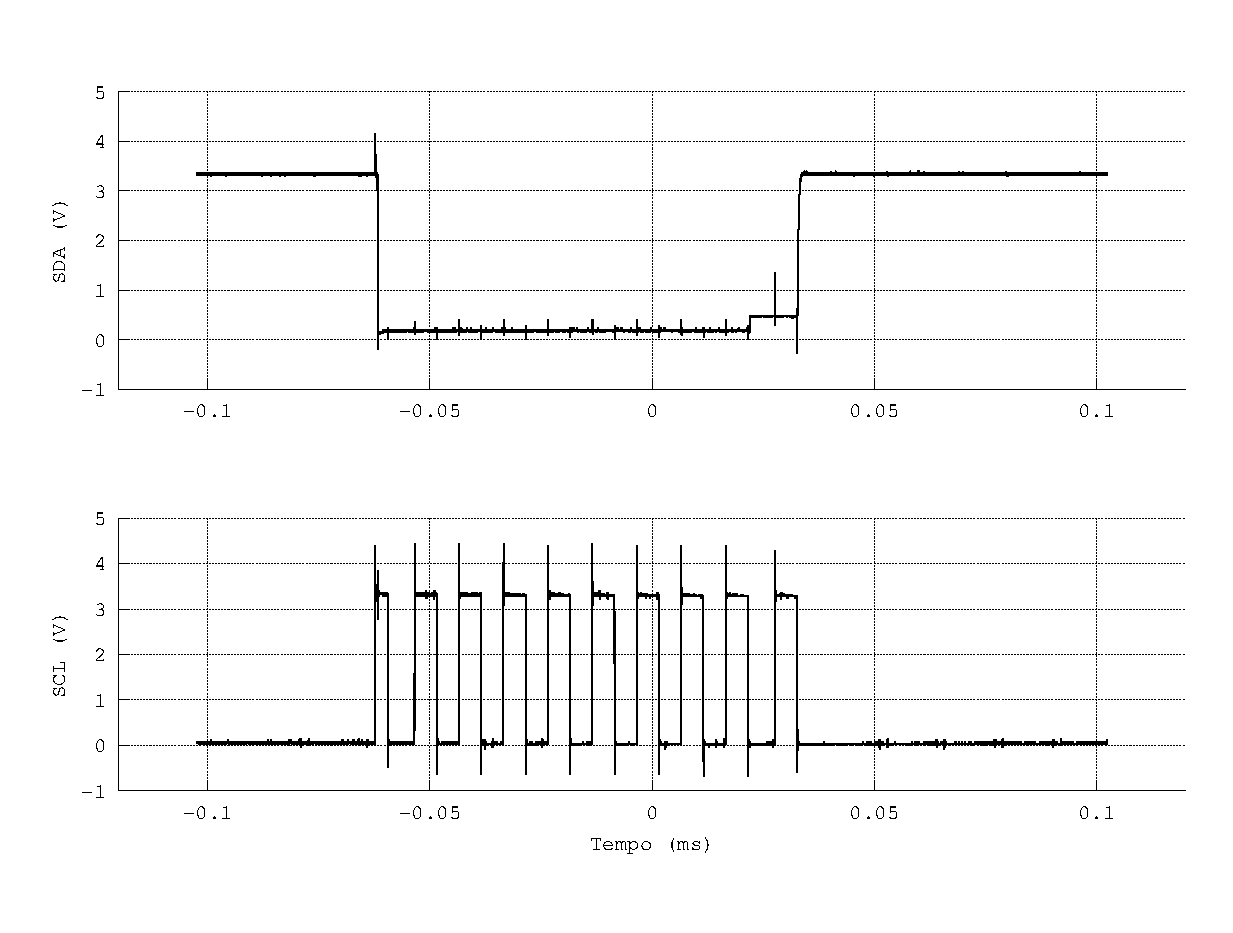
\includegraphics[width=.5\textwidth]{GeneralCallNero}
	\caption{General Call: il \master{} spedisce \texttt{0x00} e lo \slave{} risponde con l'\Ack{}}
    \label{fig:i2c_generalcall}
\end{figure}

\paragraph{Tensione di alimentazione}
	stabile a 3.3V.
    
\paragraph{Tensioni di {\sda} e {\scl}}
	corrette a 3.3 e 0V.

\paragraph{Resistenze di {\pullup}}
Né l'{\relsize{-.5}MSP430} né l'{\relsize{-.5}FT2232H}
sono dotati di opportune resistenze di {\pullup}
o per lo meno non sono configurati per usarle.
Le tensioni che si vedono durante i trasferimenti
sono infatti ottenute dal convertitore {\iic}-{\usb}
\emph{forzando alte} le linee,
cosa che non rispetta il protocollo {\iic}!
Si aggiunge quindi una resistenza da 1k$\Omega$
tra la linea dati e l'alimentazione.

Questa mancanza si manifestava dopo la trasmissione dell'indirizzo,
quando il \master{} (il convertitore {\relsize{-.5}FTDI})
rilasciava la linea dati.
Questa avrebbe dovuto risalire a $V_{CC}$ con la stessa ripidità
dei fronti di salita visti durante la trasmissione,
Si vedeva invece una rampa troppo poco pendente.
La causa di questo è appunto che prima era proprio il \master{}
a tirare su la linea, e il difetto era visibile soltanto
a linea rilasciata. A quel punto si assiste
alla carica della capacità parassita $C_P$
attraverso una resistenza $R_P$ troppo grande,
illustrata in \textsc{Figura~\ref{fig:i2c_rampa}}.\\

\begin{figure}
\centering
  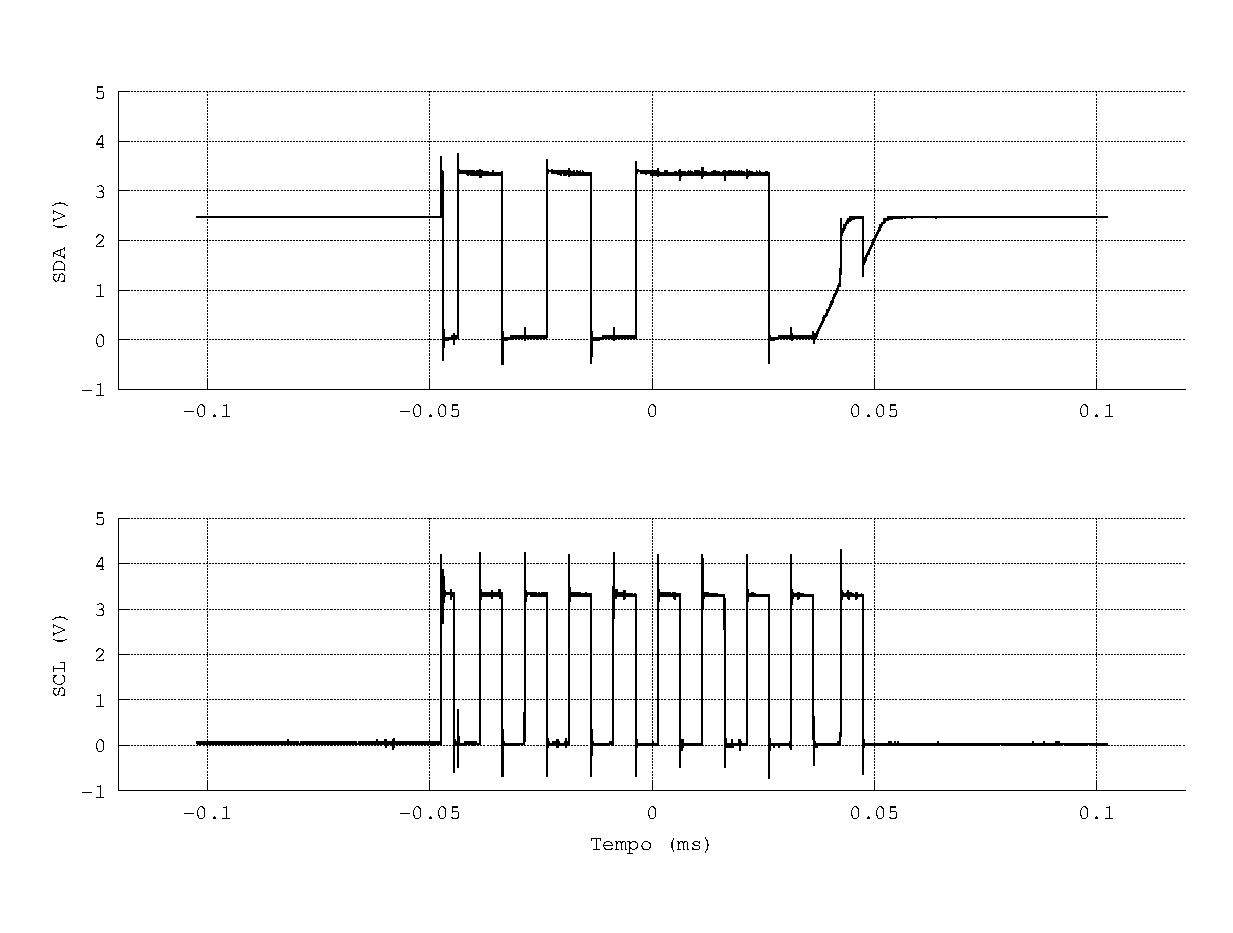
\includegraphics[width=.5\textwidth]{RampaNero}
	\caption{Senza resistenza di \pullup{}: quando il convertitore trasmette, i fronti di salita sono ripidi; quando esso rilascia la linea la tensione sale molto più lentamente.}
    \label{fig:i2c_rampa}
\end{figure}

\paragraph{Picchi di rumore}
In fase di lettura, si notano dei picchi sulla linea dati
in corrispondenza dei fronti del clock.
Questo sarà colpa della capacità parassita
tra le linee $C_C$ di \textsc{Figura~\ref{fig:i2c_tipica}}.\\

\paragraph{Ricapitolando}
Le cause della mancata ricezione degli \Ack{}
e della linea dati sempre alta
riconducono a soglie di tensione non raggiunte o picchi,
che portano all'errata interpretazione dei messaggi
e alla perdita di sincronia.
% {Resta da verificare che questi dispositivi
% non siano sensibili a combinazioni sbagliate di $R_S$ ed $R_P$
% a causa di errate soglie di tensione,
% e sensibili a interferenze e rumore
% a causa della mancanza di Trigger di Schmitt e filtri.}








